\chapter{設計}
\label{chap:wakaruland}

本章では,大勢の人がいる状況での計算機を用いたコミュニケーションの支援や
IoT時代の情報視覚化について分析し、
本論文で提案する視覚化システム『わかるらんど』の設計指針と特徴、
アプリケーションのデザインについて述べる。

\newpage

\section{『わかるらんど』のねらい}
\label{nerai}

近年,学会などでタイムライン表示のテキストチャットが
利用される機会が増えている\cite{goto2012}.
学会チャットシステムを利用すると,
発表中に参加者が意見交換したり疑問を表明したりできるといった利点があるが,
以下のような問題も存在する.

\begin{itemize}
\item 多数の人間が同時に投稿すると投稿内容がすぐに見えなくなってしまう
\item 投稿の多いアクティブな人ばかりが目立ってしまい,消極的な参加者は議論に参加しにくい
\end{itemize}

一般に,会議などで特定の人だけが沢山発言するのはよくあることであるが,
誰もが気軽に意見を表明できる環境を構築できれば有意義であろう.

日本ソフトウェア科学会主催の
WISS(Workshopn on Interactive Systems and Software)コンファレンス\footnote{\textsf{http://wiss.org/}}では,
学会が提供するチャットシステムに参加者がログインして議論するのが恒例になっており\cite{wiss_challenge},
2009年以降のWISSコンファレンスでは「On-Air Forum」\cite{nishida2011}という学会チャットシステムが利用されている.

しかし,WISS2009の実証実験によれば,
全参加者の半分弱しかログインして1回以上発言していなかった.
またWISS2015では,252アカウントが1回以上発言し総発言数は2,948回であったが,
発言数上位20\%の50アカウントによる発言が
総発言数の78.1\%にあたる2,305回を占めていた(図\ref{wisschat}).
発言数が10回未満のアカウントは190アカウントで,これは全アカウントの75.3\%にあたる.
図\ref{powerlaw}のようにアカウントと発言数は冪分布になっており,
特定の人ばかりが発言して,発言しない人は全く発言しない傾向が顕著に現れている.

\begin{figure}[h]
\centering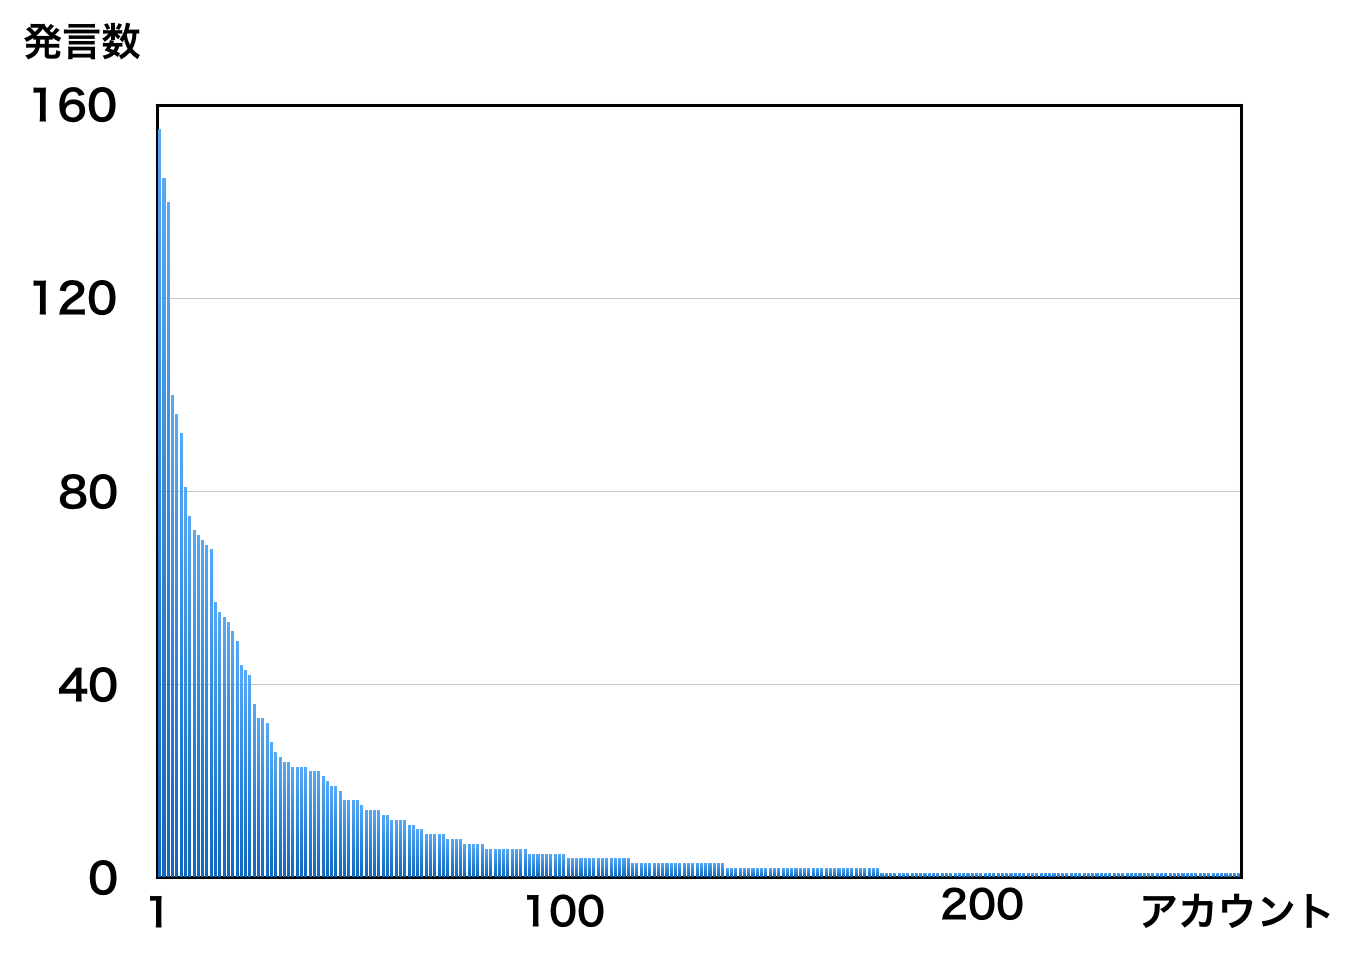
\includegraphics[width=8cm]{images/wisschat.png}
\caption{WISS2015のチャットにおけるアカウントと発言数の分布}
\label{wisschat}
\end{figure}

\begin{figure}[h]
\centering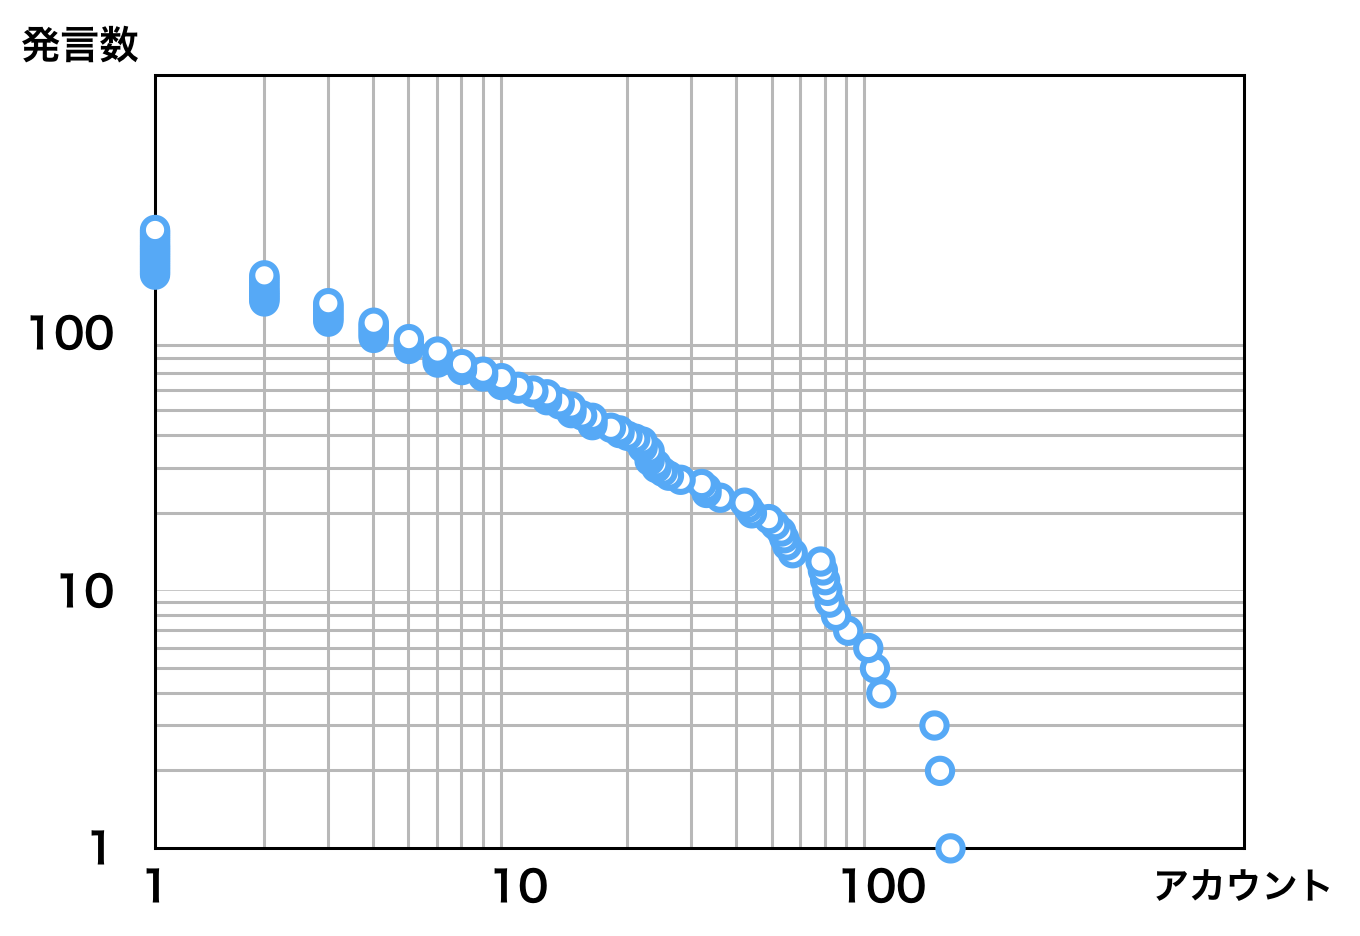
\includegraphics[width=8cm]{images/powerlaw.png}
\caption{図\ref{wisschat}の両対数グラフ}
\label{powerlaw}
\end{figure}

『わかるらんど』はユーザの表示領域が均等に決まっているため,
タイムライン表示のように投稿数が多い人ばかりが目立つということがない.
また,長いテキストを入力すると表示される文字が小さくなるので,
多数の人間で利用すると長い文字は小さすぎて読めない.
必然的にユーザは図\ref{wakaruland150}のように短文を入力することを強いられる.
『わかるらんど』では長文の高度な発言は期待しておらず,
「なるほど」「わからん」「笑」などといった相槌のようなものを
視覚化してひと目で把握できるようになることを期待している.
学生,教員,企業の研究者など様々なバックグラウンドの人が入り混じった状況で
「下手な発言ができない」「気の利いたことを言わなければならない」という
投稿を躊躇させる要素を限りなく減らし,
本当は議論に参加したいけど声が出ない/手を上げる勇気がない人でも
「なるほど」「わかる」などを『わかるらんど』に投稿することで「参加」することができる.
テキストで記述すると長くなってしまう内容も
画像スタンプを投稿することで分かってもらうことができると考える.

%\comment{
%また,長いテキストを投稿するには適していないので『わかるらんど』を使って議論することは難しいが,
%多くの会議やコンファレンスでは発表後に議論の時間が設けられているため議論はその時に行えばよい.
%}

\begin{figure}[h]
\centering
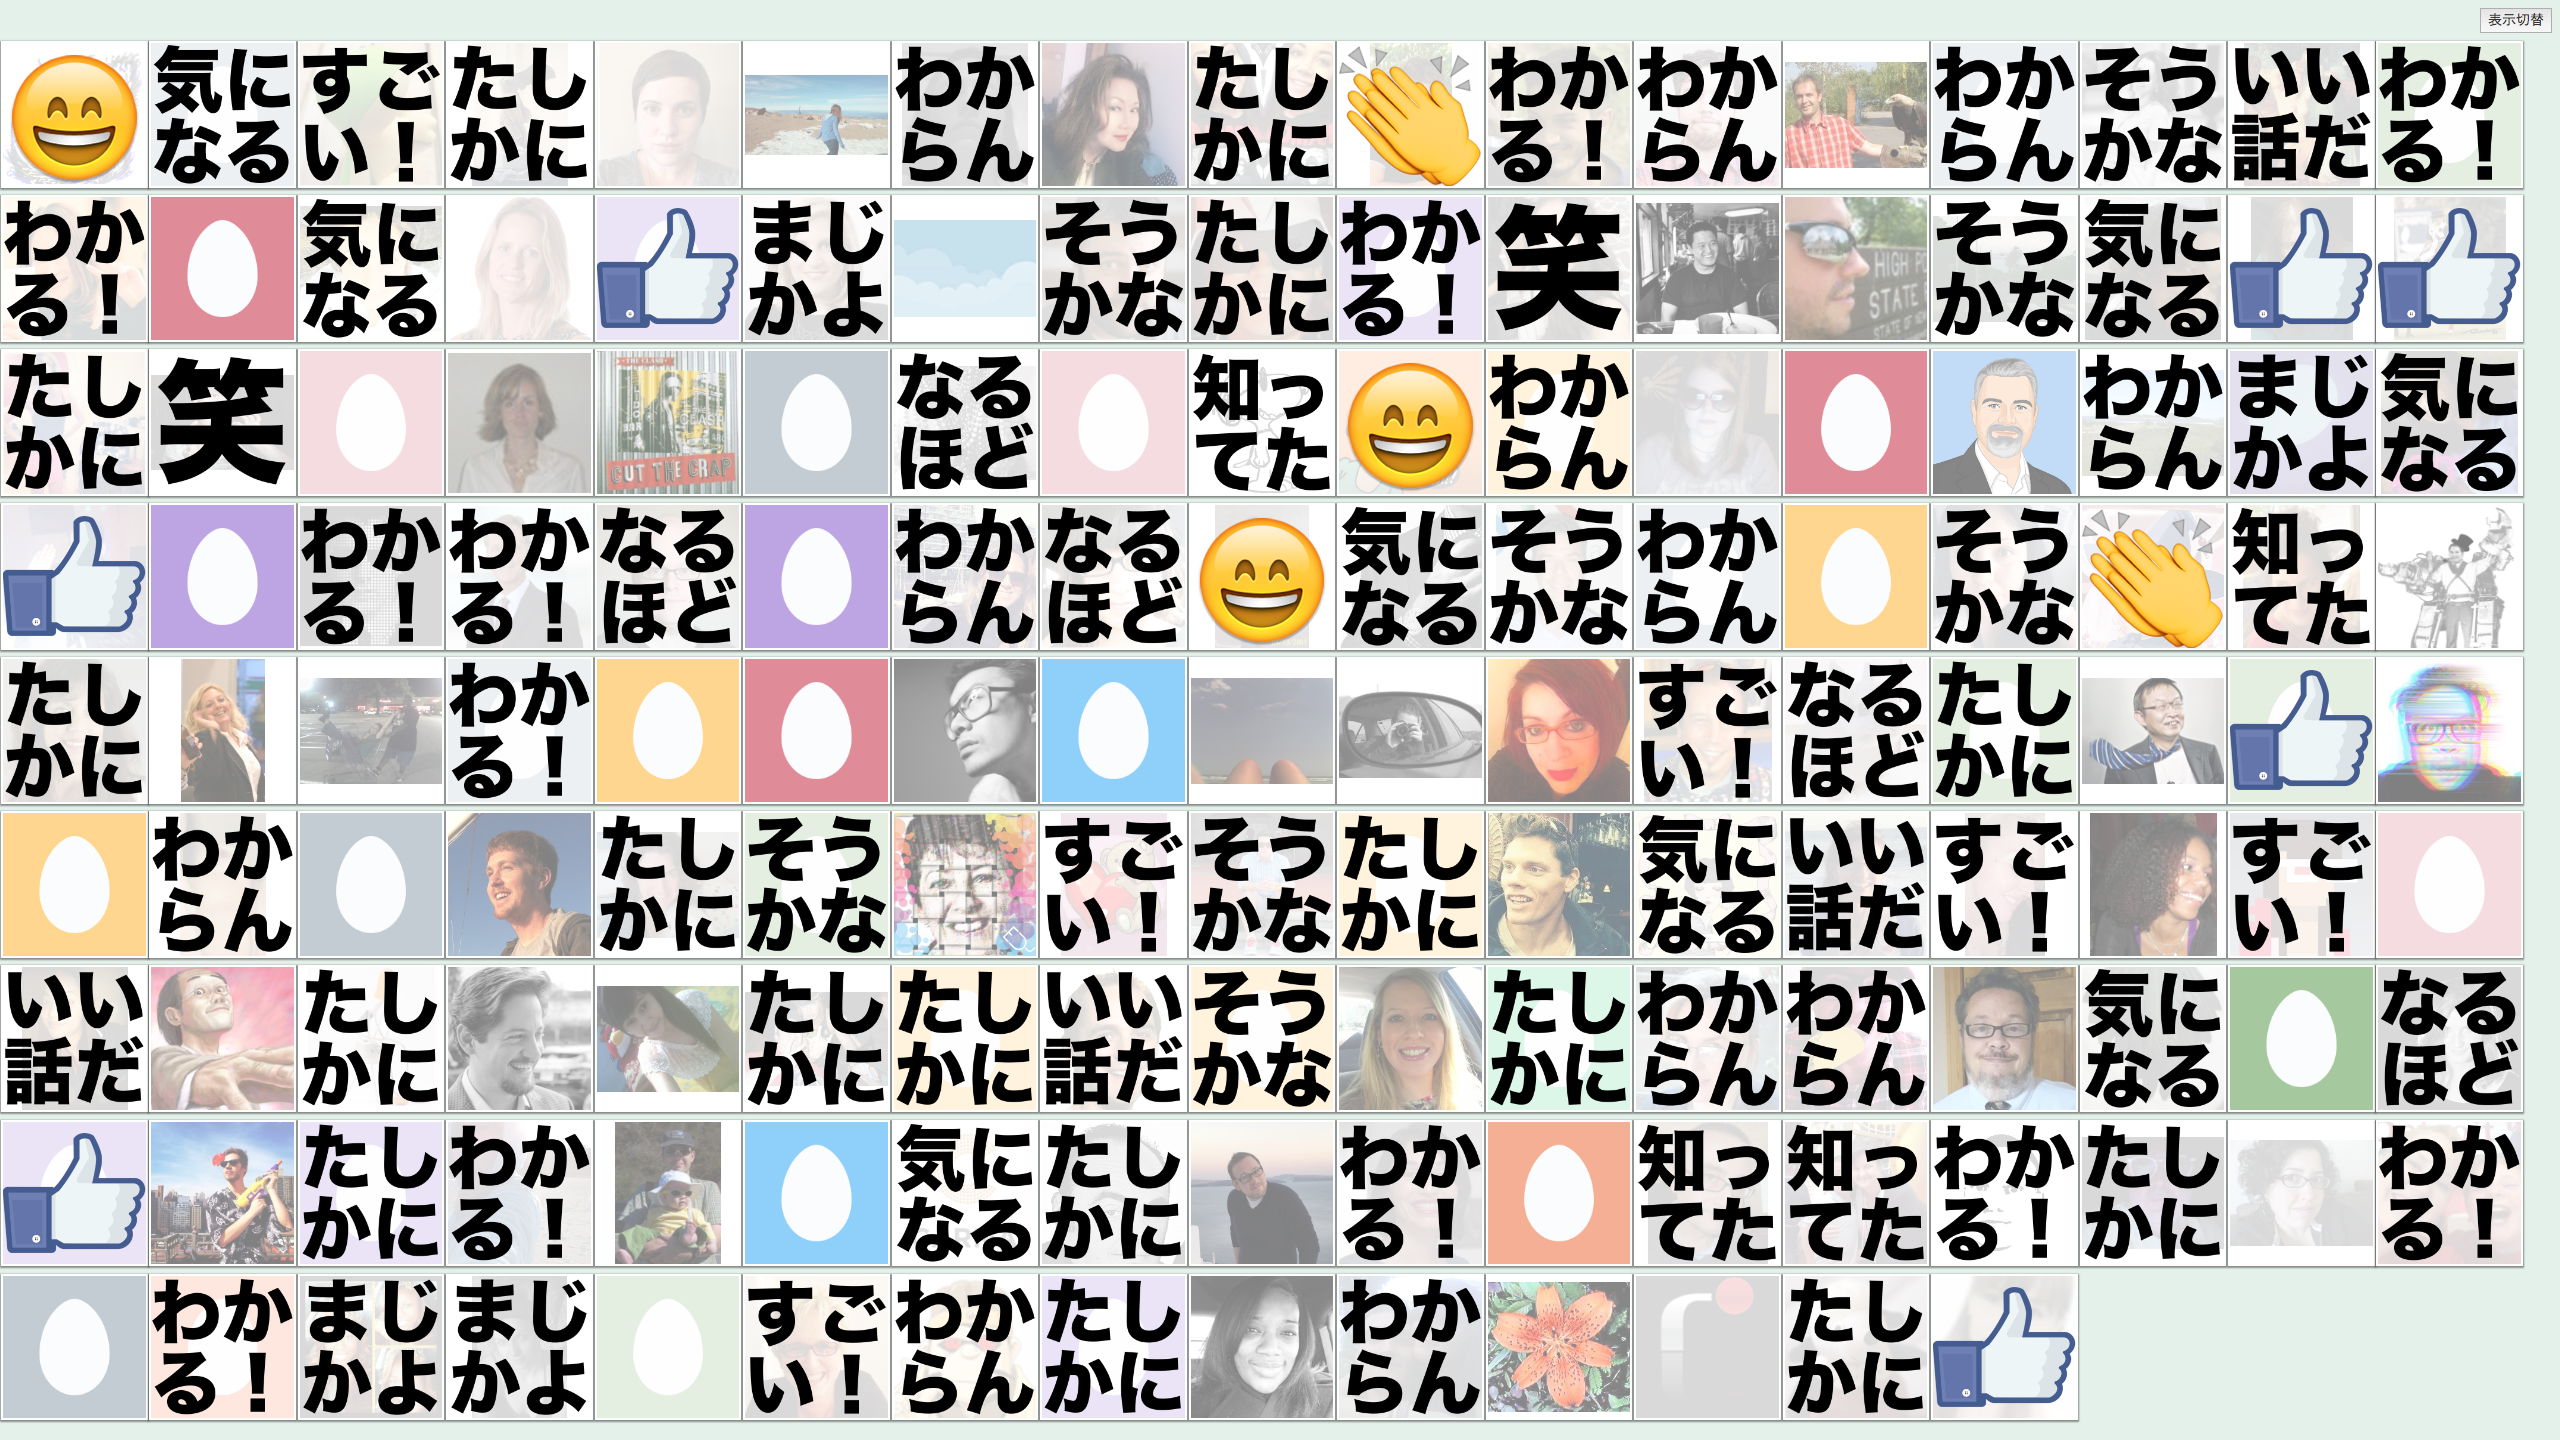
\includegraphics[width=8cm]{images/wakaruland150.png}
\caption{150人で『わかるらんど』を使用したイメージ}
\label{wakaruland150}
\end{figure}

\section{ユーザインタフェース}

『わかるらんど』のユーザインタフェースは「ダッシュボード」と「投稿画面」の2つからなり,
画面右上のボタンで切り替えることができる.
図\ref{dashboard}はダッシュボードのスクリーンショットである.
ユーザが投稿したテキストやスタンプや,
各種のセンサのデータなどがリアルタイムに1つの画面に表示されている.
センサのデータなどは自動的に更新され,ユーザのリアクションは図\ref{console}の投稿画面で
ユーザ名を入力し,スタンプを一覧から選んで投稿することで
自分のアイコンの上にオーバーレイ表示される.
ユーザの投稿には表示時間が設定されており,
指定時間が経過すると自動的に投稿が取り下げられるため
いつまでも古い投稿が表示され続けてしまうということはない.
表示時間はユーザがスタンプをクリックする時間の長さで設定される.

% 投稿するスタンプは投稿画面でユーザが自由に追加/削除することができる.

\begin{figure}[h]
\centering
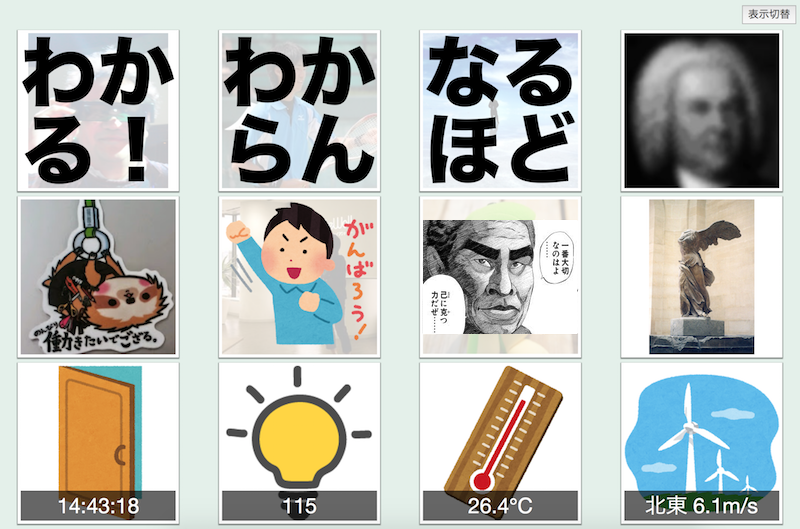
\includegraphics[width=9cm]{images/dashboard.png}
\caption{『わかるらんど』のダッシュボード}
\label{dashboard}
\end{figure}

\begin{figure}[h]
\centering
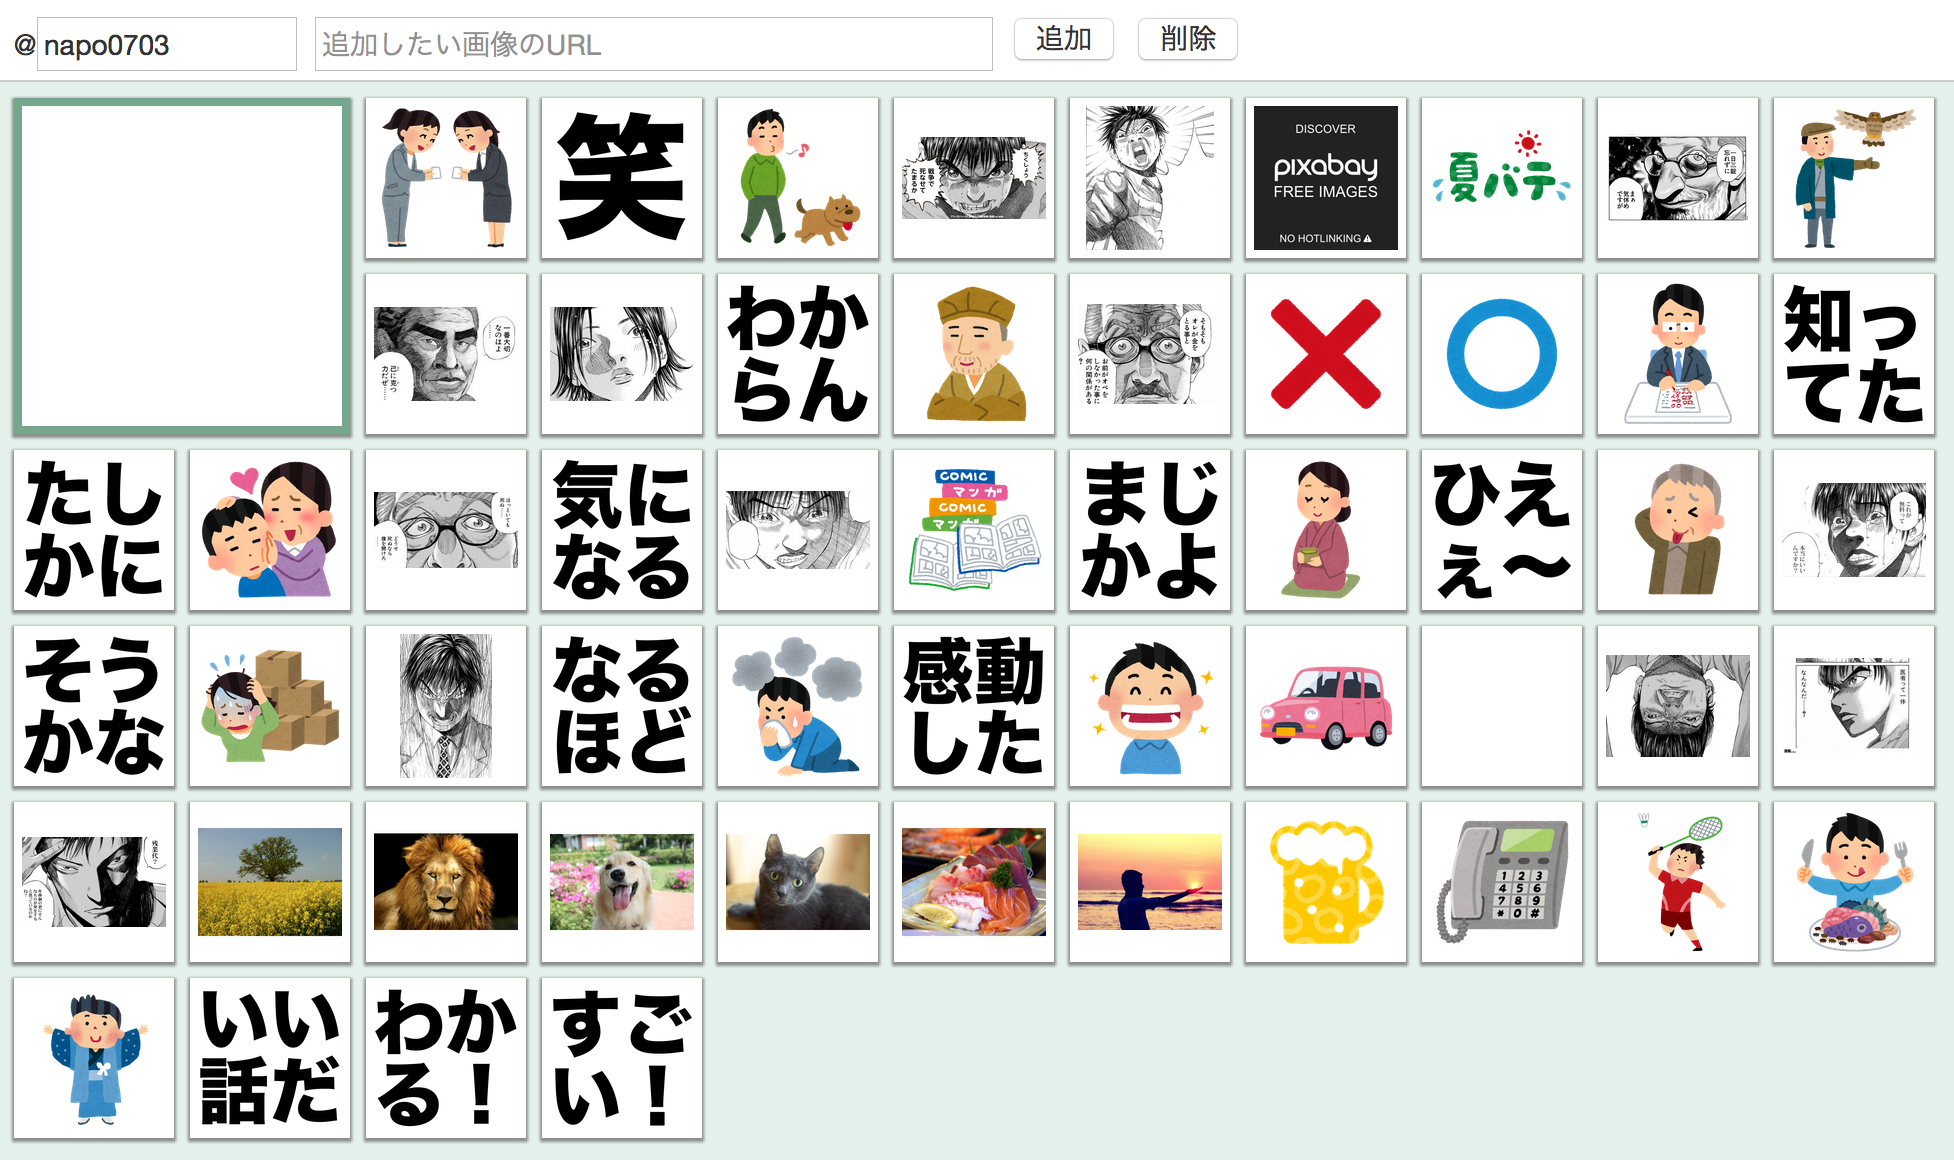
\includegraphics[width=9cm]{images/console.png}
\caption{『わかるらんど』の投稿画面}
\label{console}
\end{figure}

\section{表示するユーザとデータの指定}

『わかるらんど』のダッシュボードに表示されるセルは,ユーザのテキストや画像のスタンプを表示する
「リアクション」セルと,センサやWebの情報を表示する「データ」セルの2種類がある(図\ref{cell}).

\begin{figure}[h]
\centering
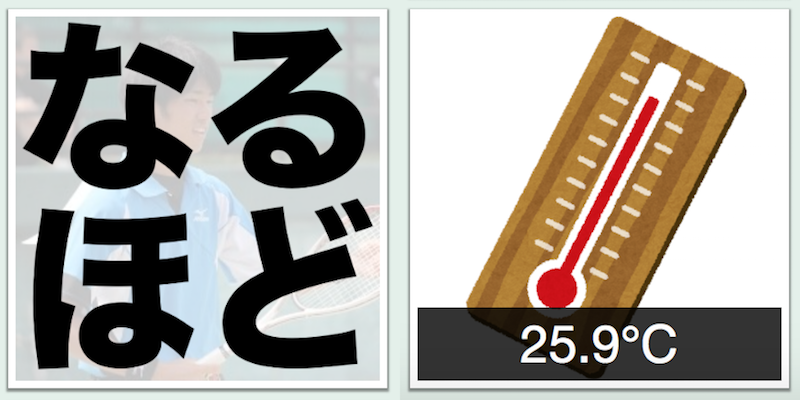
\includegraphics[width=9cm]{images/cell.png}
\caption{リアクション(左)とデータ(右)}
\label{cell}
\end{figure}

ダッシュボードに表示するユーザのリアクションの指定は,
\url{https://wakaruland.com/@napo0703,@masui,@shokai,@dorayaki0}
のようにURLの末尾にカンマ区切りでTwitterのユーザ名を「\url{@}」を付けて書くことで行う.
この場合は図\ref{n_m_s_d}のように\url{@napo0703,@masui,@shokai,@dorayaki0}の4人のユーザのセルが
ダッシュボードに表示される.

\begin{figure}[h]
\centering
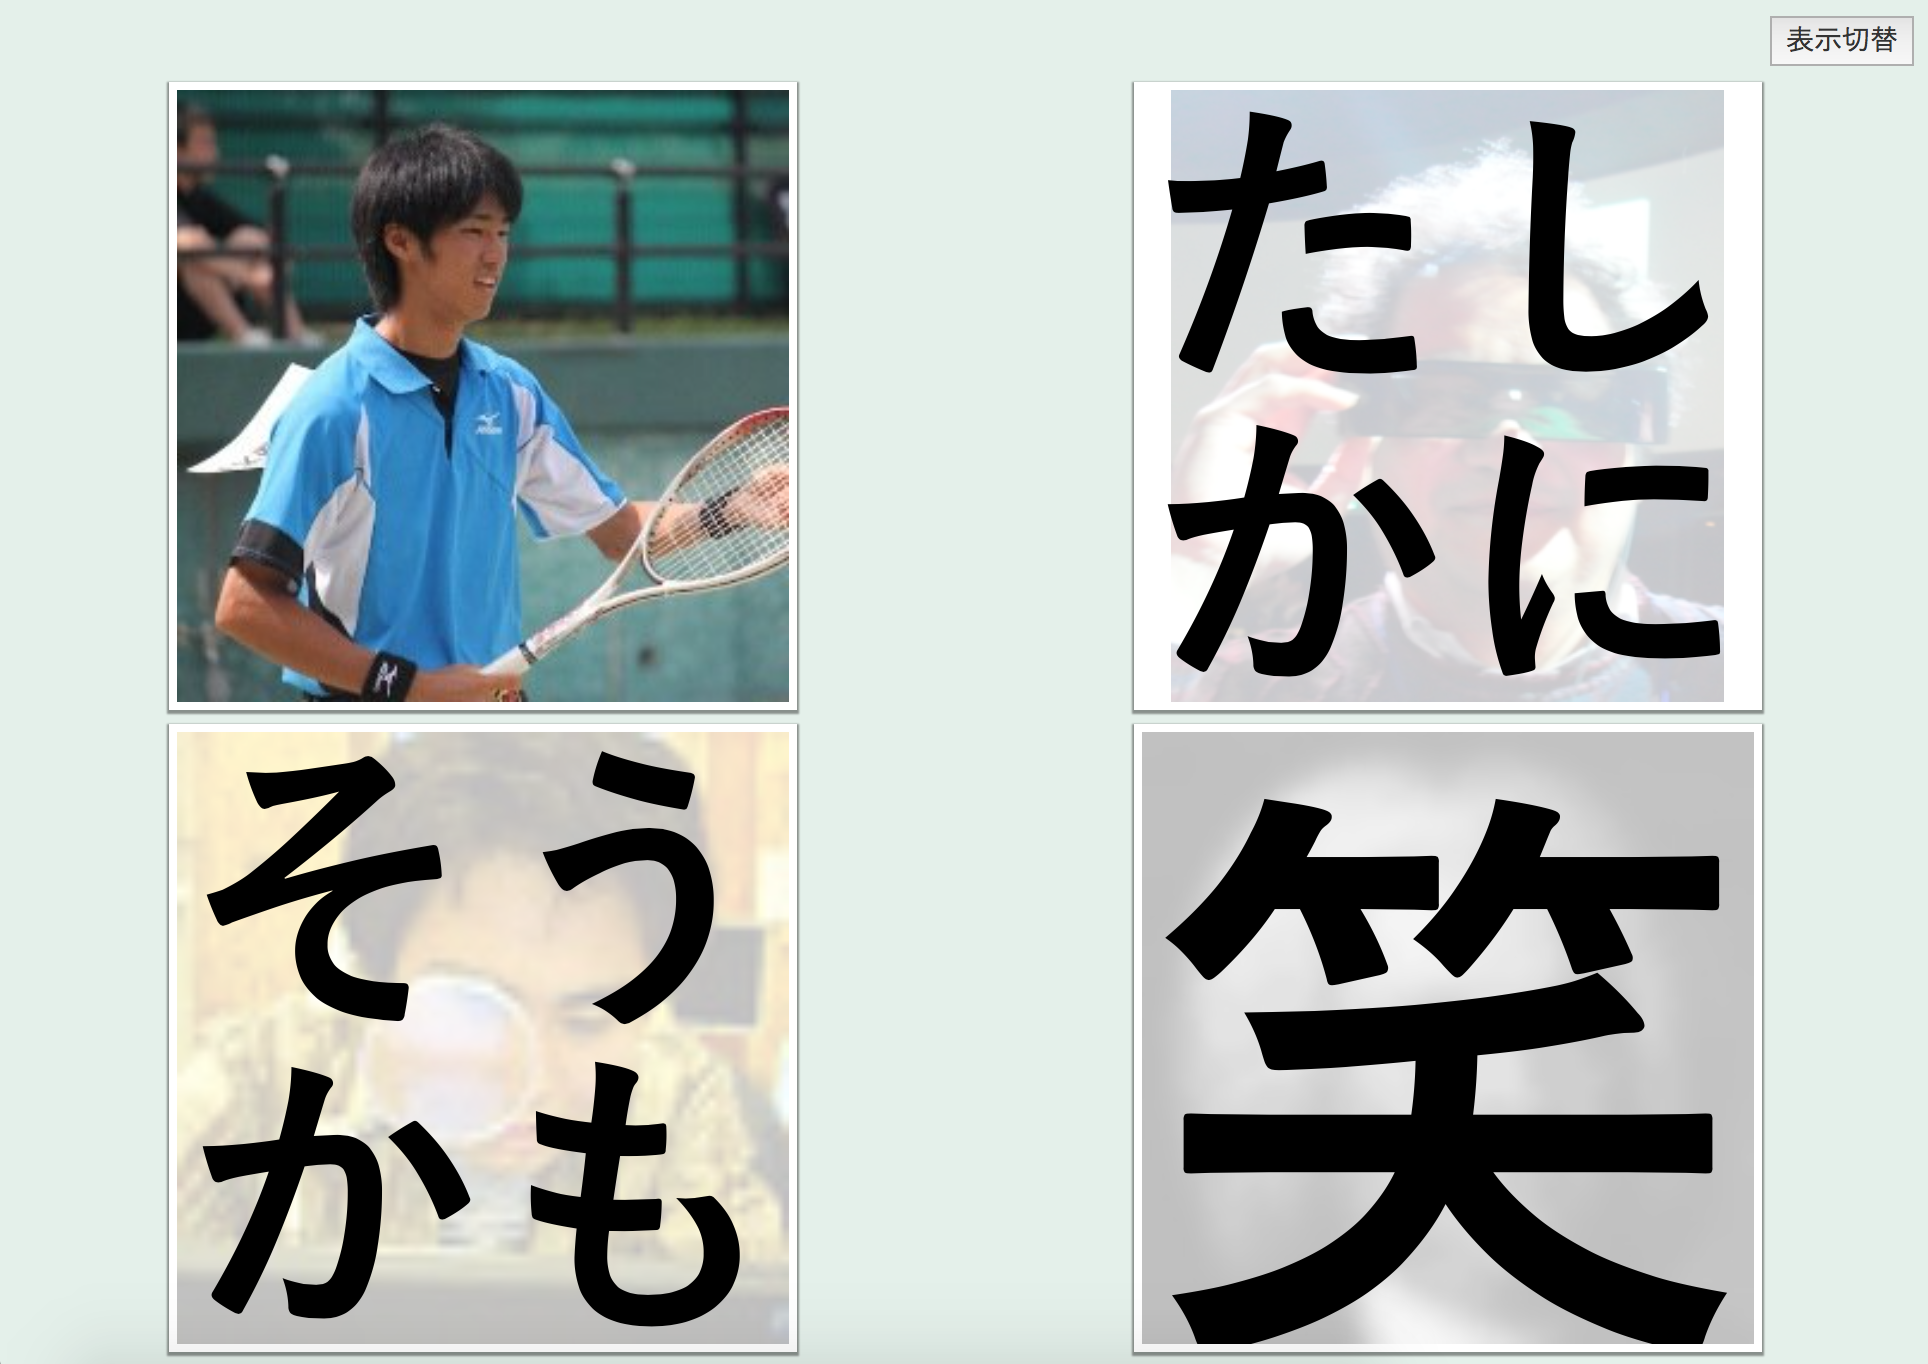
\includegraphics[width=9cm]{images/n_m_s_d.png}
\caption{4人のユーザを表示}
\label{n_m_s_d}
\end{figure}

\url{https://wakaruland.com/weather,temperature,wind}のように「\url{@}」を付けなかった場合は図\ref{w_t_w}のように\url{weather,temperature,wind}の3つがデータのセルとして表示される.

\begin{figure}[h]
\centering
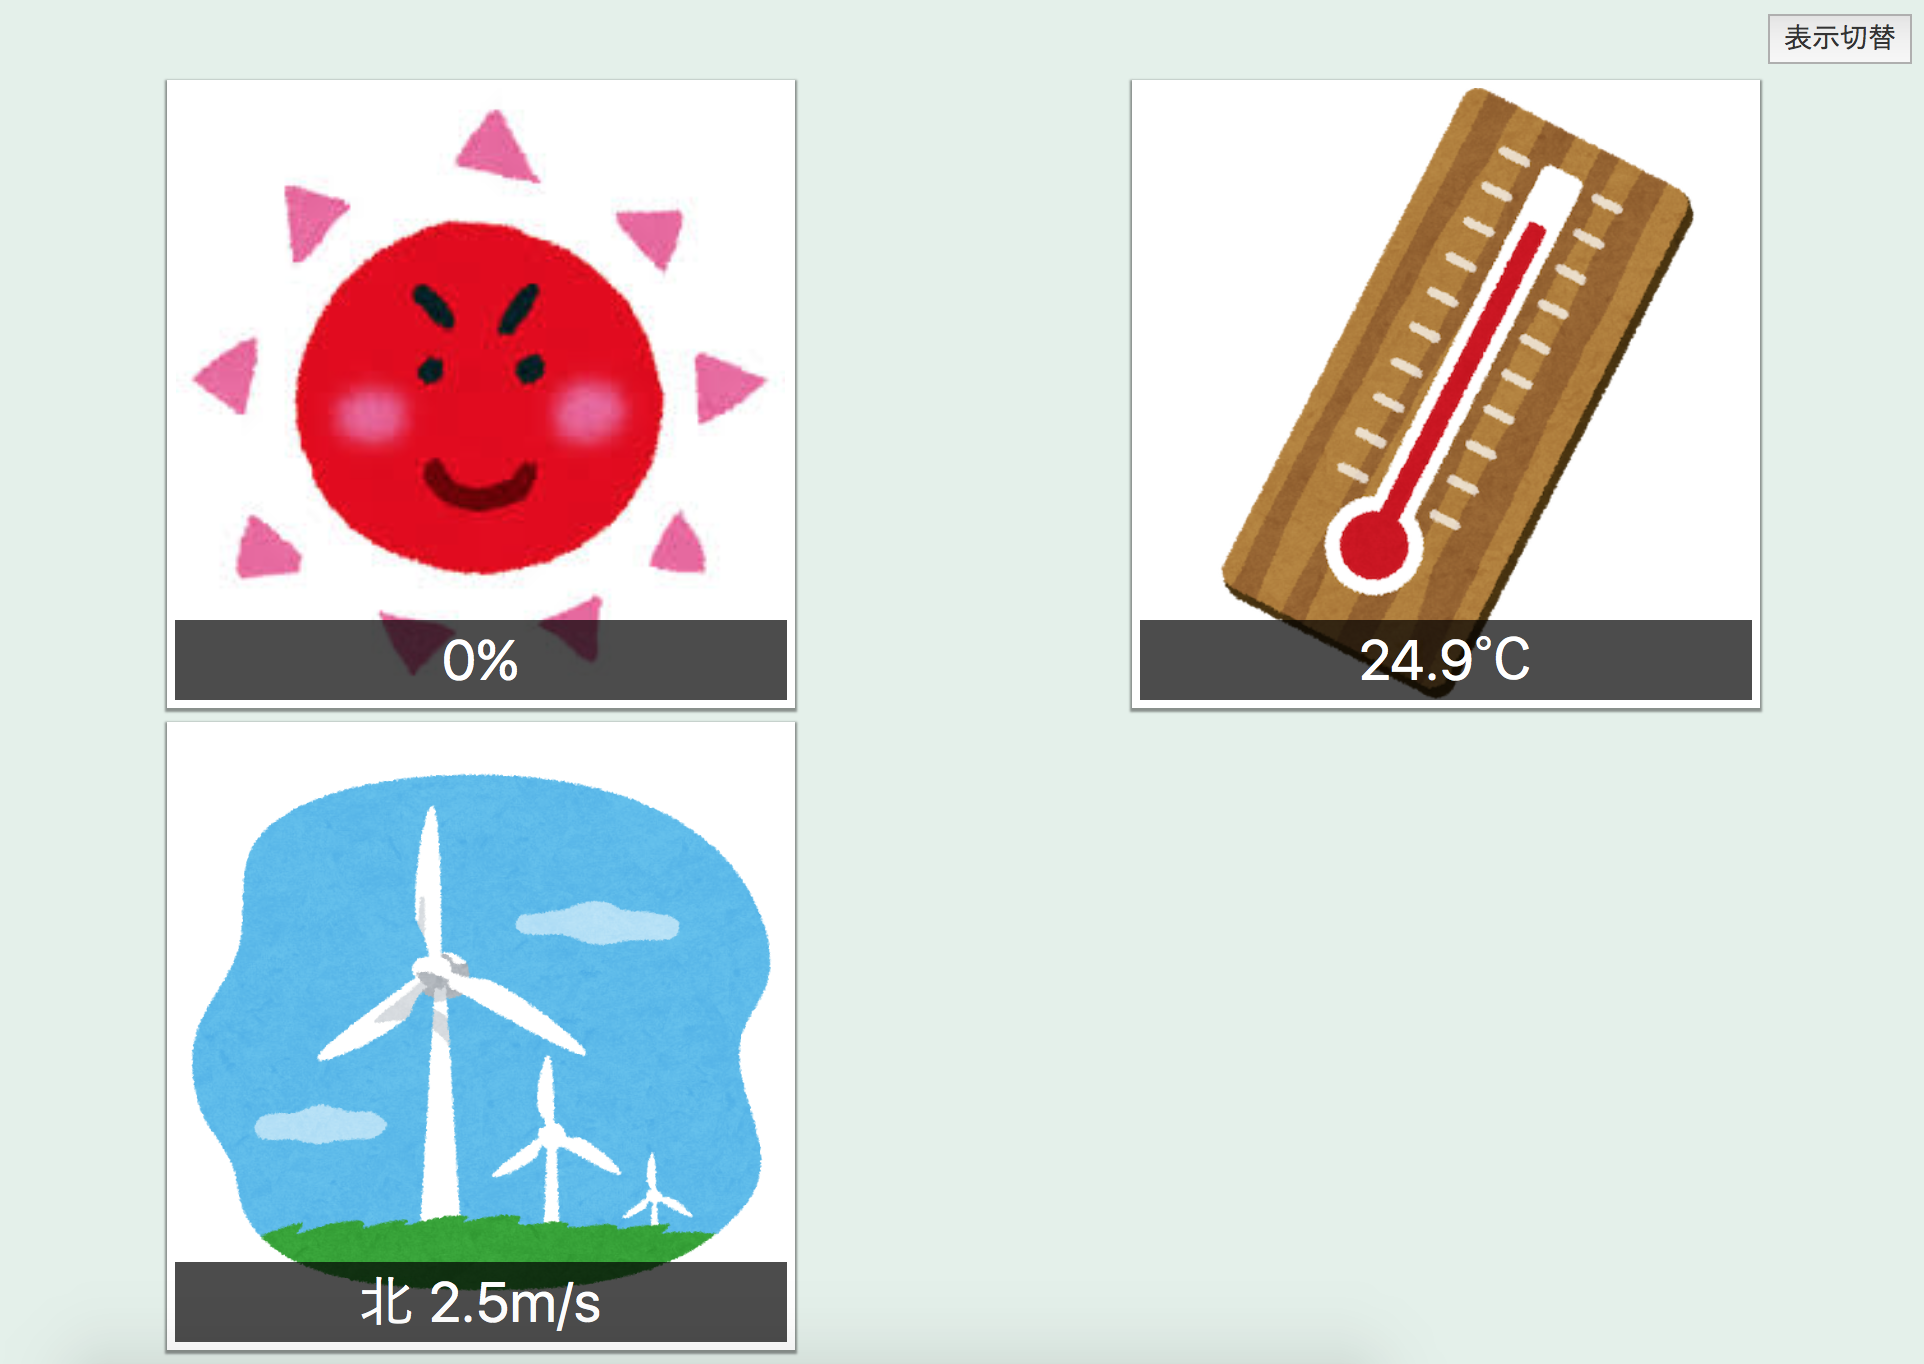
\includegraphics[width=9cm]{images/w_t_w.png}
\caption{3つのデータを表示}
\label{w_t_w}
\end{figure}

また,\url{https://wakaruland.com/@napo0703,weather,@masui,wind,@shokai}のようにリアクションとデータを合わせて表示させることも可能である(図\ref{n_w_m_w_s}).

\begin{figure}[h]
\centering
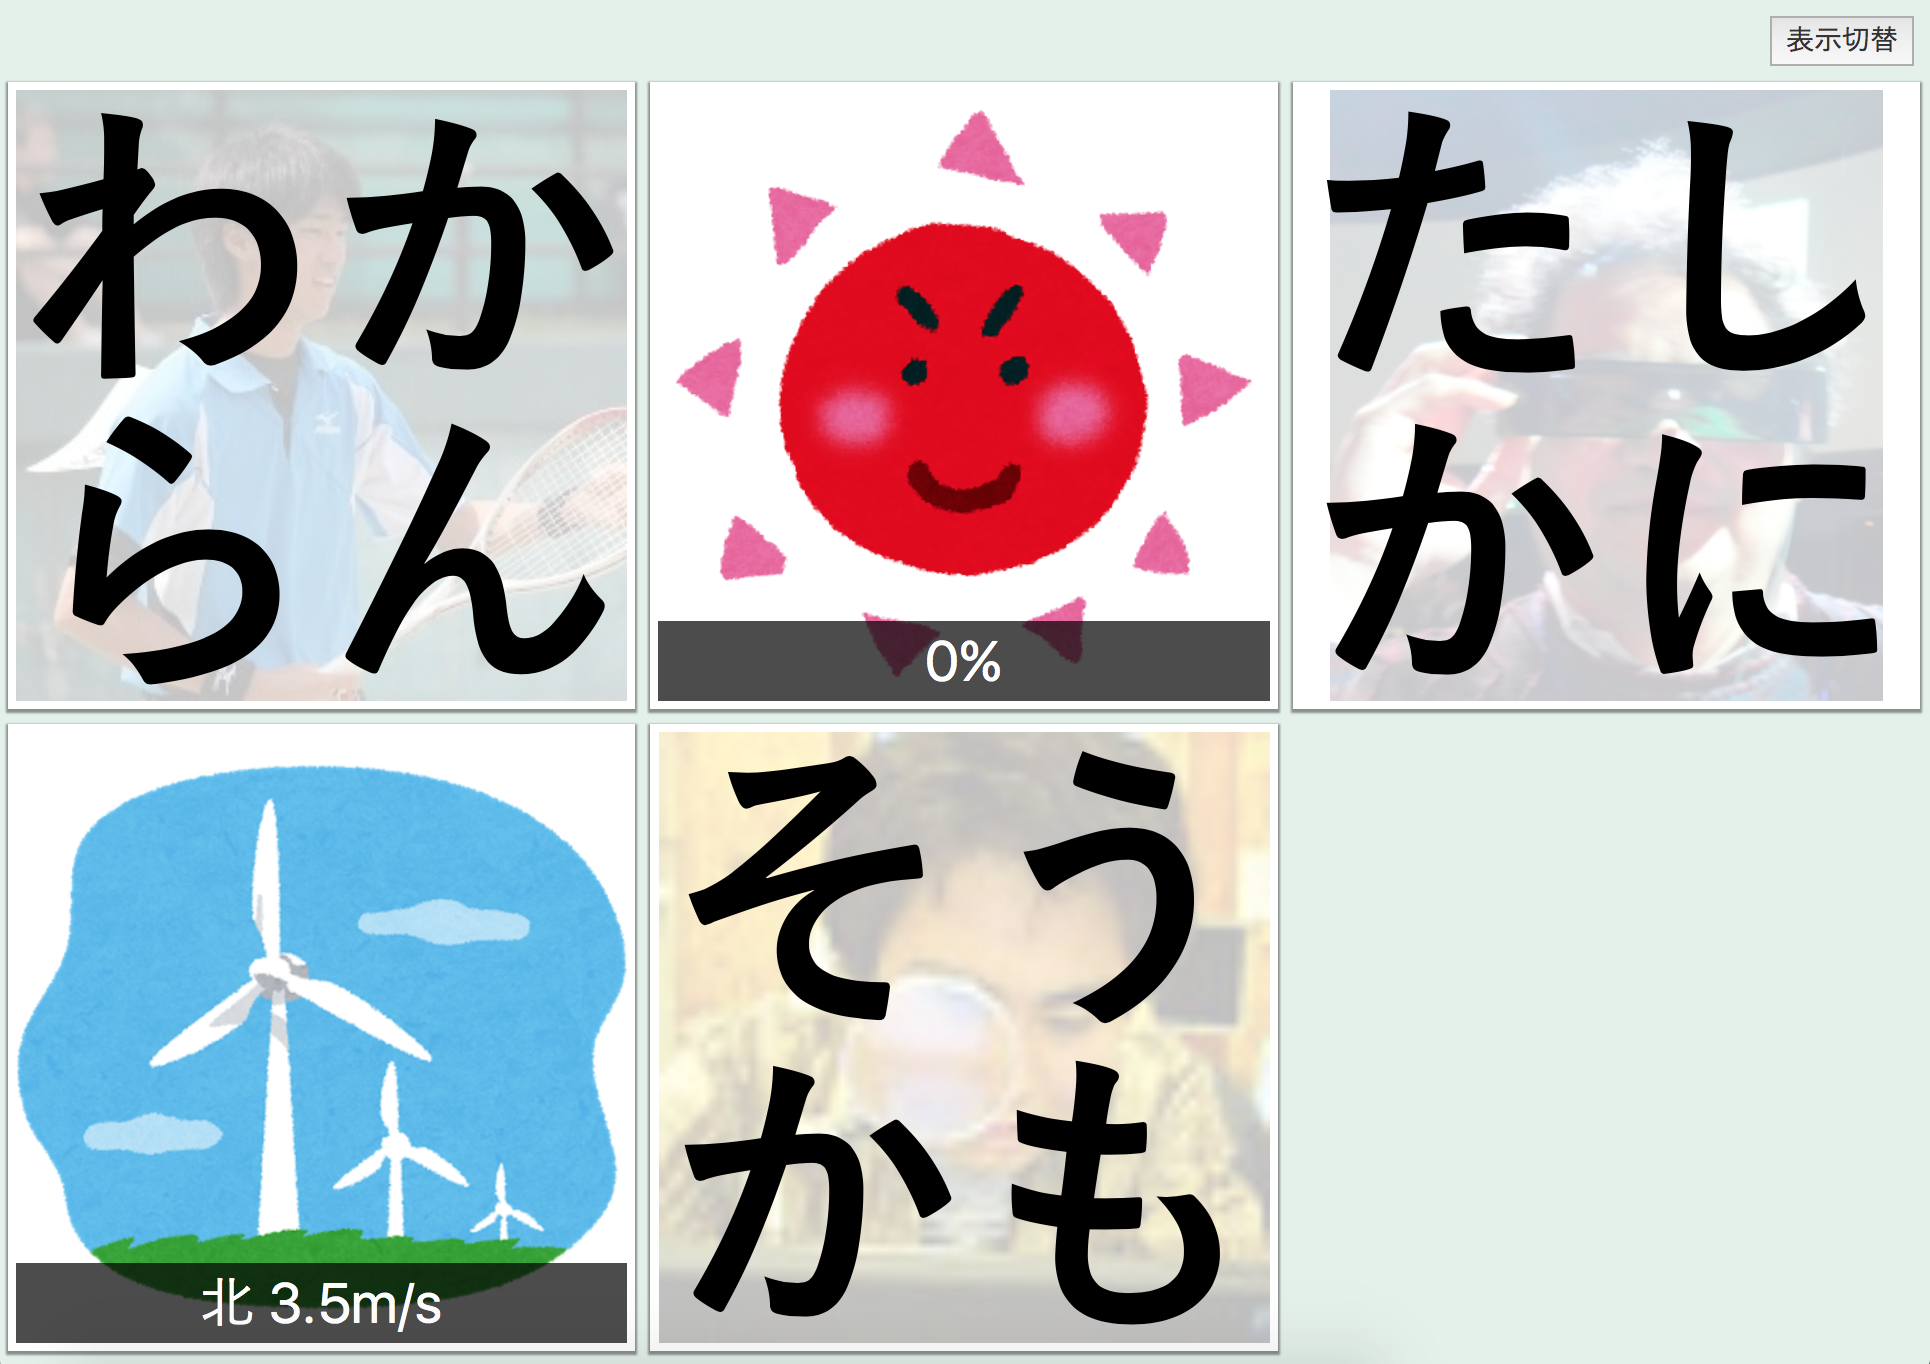
\includegraphics[width=9cm]{images/n_w_m_w_s.png}
\caption{ユーザとデータを表示}
\label{n_w_m_w_s}
\end{figure}

\section{スタンプの作成}
ユーザが投稿画面でリアクションとして投稿するスタンプには,
「テキスト」スタンプと「画像」スタンプの2種類がある(図\ref{stamp}).

ユーザは投稿画面のテキストボックスに文字列を入力して追加ボタンを押すことで
スタンプを作成して追加することができる.

画像スタンプは,テキストボックスに\url{http://masuilab.org/image.jpg}のようなWebにある
画像のURLを入力し追加ボタンを押すことで,URLの画像をスタンプとして一覧に追加することができる.
ローカルにある画像ファイルをスタンプとして追加したい場合は,
Gyazo\footnote{https://gyazo.com}などのアプリケーションを使って
WebにアップロードしURLを得ることで追加が可能である.

テキストスタンプは,テキストボックスにURLでないを文字列を入力し追加ボタンを押すことで作成できる.
図\ref{wakaran}左は「わからん」とテキストボックスに入力してスタンプを作成したものである.
この「わからん」は1行に表示されているが,「わか らん」と改行を入れたい場所に空白文字を入力
することで,図\ref{wakaran}右のように2行で表示される.

% スタンプの削除は,スタンプにマウスオーバーすると右上に表示される「×」ボタンを押すことで削除できる.

\begin{figure}[h]
\centering

\includegraphics[width=9cm]{images/stamp.png}
\caption{テキストスタンプ(左)と画像スタンプ(右)}
\label{stamp}
\end{figure}

\begin{figure}[h]
\centering
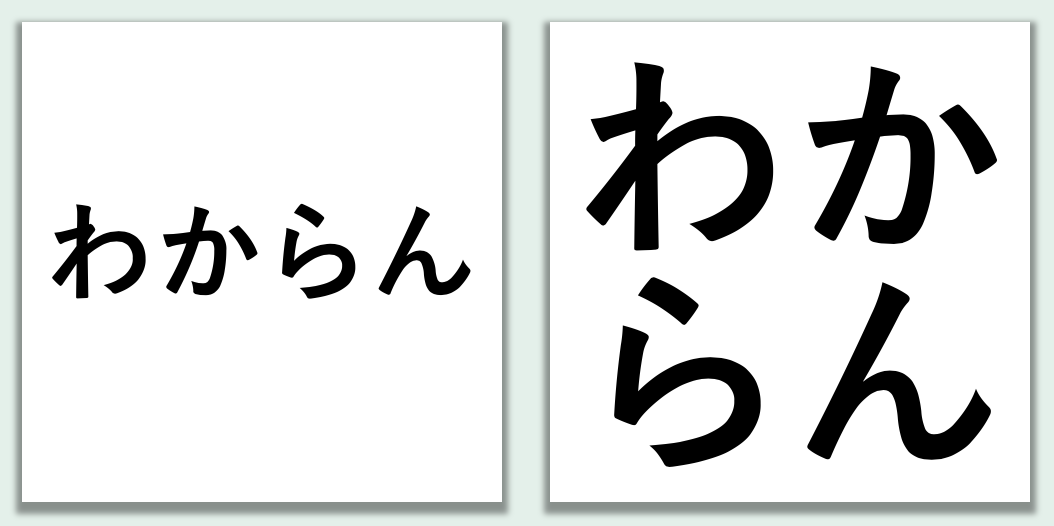
\includegraphics[width=9cm]{images/wakaran.png}
\caption{「わからん」スタンプ(左)と「わか らん」スタンプ(右)}
\label{wakaran}
\end{figure}

\section{利用例}
図\ref{discussion}は会議や発表の場での利用例である.これは誰かが何か変なことを言ったのに対してユーザが反応している様子である.

図\ref{sensors}はダッシュボードとしての利用例で,
各種のセンサの値やWebの情報等を表示している.
データはリアルタイムに最新のものに更新されていく.

\begin{figure}[h]
\centering
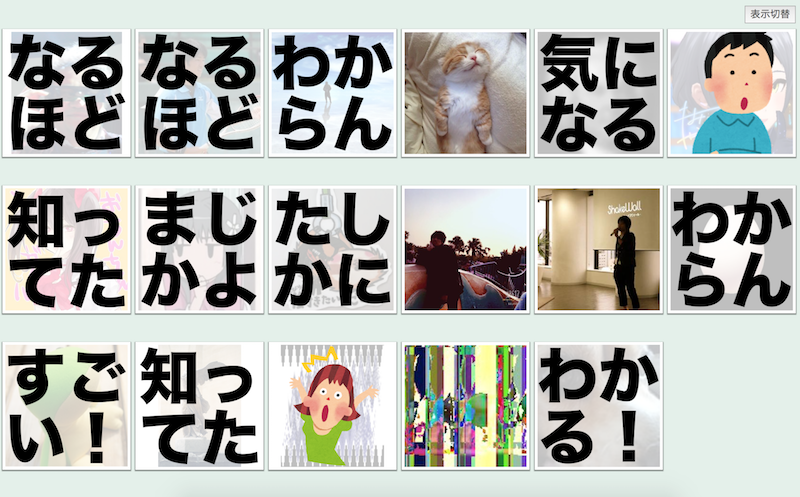
\includegraphics[width=9cm]{images/discussion.png}
\caption{会議や発表の場での利用例}
\label{discussion}
\end{figure}

\begin{figure}[h]
\centering
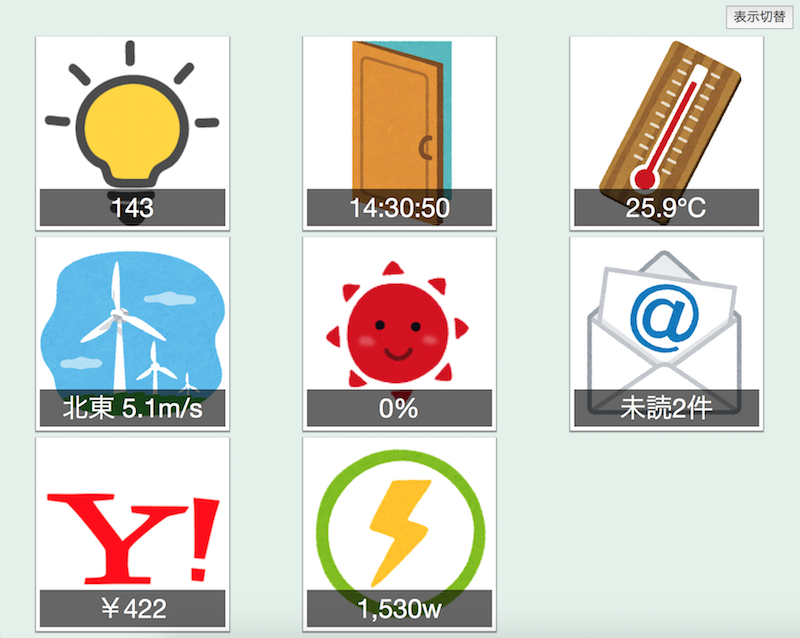
\includegraphics[width=9cm]{images/sensors.png}
\caption{ダッシュボードとしての利用例}
\label{sensors}
\end{figure}